\documentclass[a4paper, 12pt, final, garamond]{book}
\usepackage{cours-preambule}

\raggedbottom

\makeatletter
\renewcommand{\@chapapp}{\'Electrocin\'etique -- chapitre}
\makeatother

\begin{document}
\setcounter{chapter}{1}

\chapter{TD~: circuits \'electriques avec r\'esistances et sources}

\section{Circuit simple}
On constitue un circuit électrique avec un générateur réel de tension $(E,r)$,
entre les bornes duquel on branche une résistance $R$ réglable.

\begin{enumerate}
    \item Faire un schéma normalisé du circuit.
    \item Flécher les tensions et intensités, en respectant la convention pour
        chacun.
    \item Déterminer l'expression de l'intensité du courant qui circule dans le
        circuit.
    \item Déterminer l'expression de la puissance absorbée par la résistance.
    \item Tracer la courbe de $P$ en fonction de $R$, et montrer que cette
        courbe passe par un maximum. Déterminer les coordonnées du maximum.
\end{enumerate}

\section{Résistances équivalentes}
\begin{enumerate}
    \item Exprimer la résistance équivalente à l'association de deux résistances
        $R_1$ et $R_2$ placées en parallèle.
    \item Que devient cette expression si $R_1 = R_2$~?
    \item Exprimer la résistance équivalente à l'association d$e_3$ résistances
        $R_1$, $R_2$ et $R_3$ placées en parallèle.
    \item Que devient cette expression si $R_1 = R_2 = R_3$~?
    \item Exprimer la résistance équivalente à l'association de $n$ résistances
        identiques placées en parallèle.
\end{enumerate}

\section{Association de générateurs}
Deux générateurs de tension de forces électromotrices $E_1$ et $E_2$ et de
résistances internes $r_1$ et $r_2$ sont branchés en série. Ils alimentent une
résistance $R_3$.

\begin{enumerate}
    \item Dessiner le schéma normalisé de ce circuit électrique et flécher les
        courants et les tensions.
    \item Écrire l'équation de la maille et en déduire l'expression du courant
        qui circule dans cette maille.
    \item Simplifier le schéma en ne faisant apparaître qu'un seul générateur
        équivalent aux deux générateurs initiaux aux bornes de $R_3$.
    \item Que devient le générateur équivalent lorsque $r_1$ et $r_2$ sont
        nulles~?
    \item Conclusion à retenir : peut–on brancher deux générateurs idéaux de
        tension en série~? Deux générateurs réels~?
\end{enumerate}
Les deux générateurs ($E_1$, $r_1$) et ($E_2$, $r_2$) sont maintenant placés en
parallèle. Ils alimentent une résistance $R_4$ (en parallèle sur l'ensemble des
deux générateurs).
\begin{enumerate}[resume]
    \item Dessiner le schéma normalisé de ce montage et flécher les courants et
        les tensions.
    \item Reproduire le schéma avec des générateurs idéaux (donc $r_1$ et $r_2$
        nulles) et flécher les courants et les tensions. Que peut-on dire de la
        tension aux bornes de $R_4$~?
    \item Conclusion à retenir : peut–on brancher deux générateurs idéaux de
        tension en parallèle~? Deux générateurs réels~?
\end{enumerate}

\section{Calcul de résistances équivalentes} Exprimer la résistance équivalente
entre les points $A$ et $B$ pour chacun des schémas suivants. \bigbreak

\begin{minipage}{0.32\linewidth}
    \begin{center}
        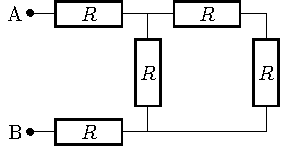
\includegraphics[width=\linewidth]{requiv_a-plain}
    \end{center}
\end{minipage}
\begin{minipage}{0.32\linewidth}
    \begin{center}
        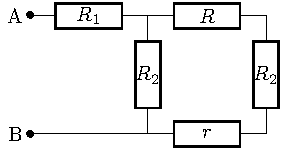
\includegraphics[width=\linewidth]{requiv_b-plain}
    \end{center}
\end{minipage}
\begin{minipage}{0.32\linewidth}
    \begin{center}
        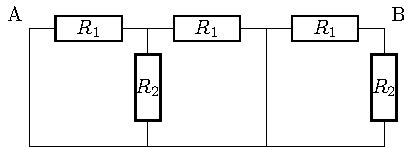
\includegraphics[width=\linewidth]{requiv_c-plain}
    \end{center}
\end{minipage}

\section{Conventions}

\begin{minipage}{0.30\linewidth}
    Pour le circuit ci-contre :
\end{minipage}
\begin{minipage}{0.70\linewidth}
    \begin{center}
        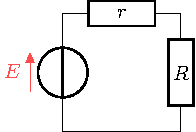
\includegraphics[width=.3\linewidth]{convs_plain}
    \end{center}
\end{minipage}
\begin{enumerate}
    \item
        \begin{enumerate}
            \item Flécher les courants et les tensions en convention récepteur
                pour chaque dipôle.
            \item Exprimer la puissance (notée P(R) pour le dipôle R) associée à
                chaque dipôle.
            \item En faisant un bilan de puissance reçue par le système,
                déterminer l'expression du courant I.
        \end{enumerate}
    \item
        \begin{enumerate}
            \item Reproduire le circuit et flécher les courants et tensions en
                convention générateur pour chaque dipôle.
            \item Exprimer la puissance associée à chaque dipôle.
            \item En faisant un bilan de puissance, déterminer l'expression du
                courant I.
        \end{enumerate}
    \item
        \begin{enumerate}
            \item Reproduire le schéma et flécher les courants et tensions de
                chaque dipôle en fonction de sa nature (récepteur / générateur).
            \item Exprimer la puissance associée à chaque dipôle.
            \item En faisant un bilan de puissance reçu par le système,
                déterminer l'expression du courant I.
        \end{enumerate}
    \item Comparer les résultats obtenus aux réponses précédentes
\end{enumerate}

\section{Mesures de tensions et intensités}

Dans les circuits ci-dessous, quelles sont les valeurs affichées par les
instruments de mesure si ceux-ci sont parfaits~? On donne : $E = \SI{5,0}{V}$ ;
$r_1 = \SI{10}{\Omega}$ ; $R = \SI{20}{\Omega}$ ; $R_1 = \SI{30}{\Omega}$ ; $R_2
= \SI{40}{\Omega}$. On rappelle que dans un circuit, les ampèremètres parfaits
sont équivalents à des fils alors que les voltmètres parfaits sont équivalents à
des interrupteurs ouverts.

\begin{minipage}{0.48\linewidth}
    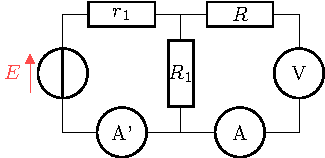
\includegraphics[width=\linewidth]{mes_iu_a-plain}
\end{minipage}
\hfill
\begin{minipage}{0.48\linewidth}
    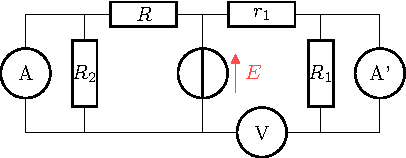
\includegraphics[width=\linewidth]{mes_iu_b-plain}
\end{minipage}

\section{Diviseur de tension}

\begin{wrapfigure}[10]{R}{.2\linewidth}
    \centering
    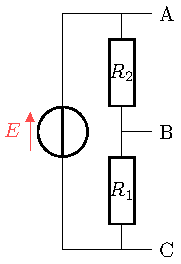
\includegraphics[width=\linewidth]{divtens_plain}
\end{wrapfigure}
~
\begin{enumerate}
    \item Écrire la loi des mailles pour le montage ci-contre et en déduire
        l'expression de l'intensité du courant $I(R_2)$ qui parcourt cette
        maille.
    \item En déduire l'expression de la tension $U_{BC}$, aux bornes de la
        résistance $R_1$.
\end{enumerate}
On ajoute une résistance $R_3$ qui sera connectée en parallèle avec la
résistance $R_1$.
\begin{enumerate}[resume]
    \item Est-ce que la valeur de la tension $U_{BC}$ calculée à la question
        précédente va changer~?
    \item Si oui, calculer les nouvelles valeurs de $U_{BC}$ et $I(R_2)$.
\end{enumerate}

\section{Diviseur de courant}

\begin{wrapfigure}[10]{R}{.2\linewidth}
    \vspace{60pt}
    \centering
    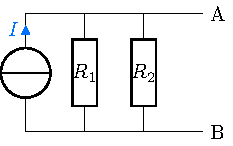
\includegraphics[width=\linewidth]{divcour_plain}
\end{wrapfigure}
~
\begin{enumerate}
    \item Exprimer les tensions aux bornes de $R_1$ et $R_2$ dans le montage
        ci-contre.
    \item A partir de la loi des mailles, exprimer $I(R_2$) en fonction de I,
        $R_1$ et $R_2$.
\end{enumerate}
On ajoute une résistance $R_3$ qui sera connectée en parallèle avec la
résistance $R_1$.
\begin{enumerate}[resume]
    \item Est-ce que la valeur de l'intensité $I(R_2$) va changer~?
    \item Si oui, donner sa nouvelle expression.
    \item Est-ce que la valeur de l'intensité délivrée par le générateur va
        changer~?
    \item Si oui, donner sa nouvelle expression.
\end{enumerate}

\section{Calcul d'intensité}

\begin{minipage}{0.45\linewidth} En utilisant les lois fondamentales dans l'ARQS
    (dites \textit{lois de Kirchhoff}), exprimer l'intensité traversant $R$ dans
    le circuit ci-contre. Faire de même avec un pont diviseur de courant d'une
    part, et de même avec un diviseur de tension d'autre part.
\end{minipage}
\begin{minipage}{0.45\linewidth}
    \begin{center}
        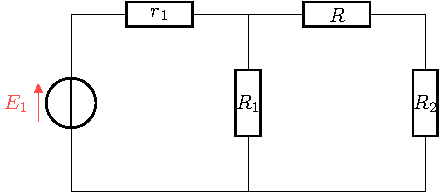
\includegraphics[width=\linewidth]{calc_intens-plain}
    \end{center}
\end{minipage}

\section{Association de générateurs~: application}

Deux générateurs de tension ($E_1$, $r_1$) et ($E_2$, $r_2$) sont placés en
parallèle l'un de l'autre. Ils alimentent une résistance $R_4$, également placée
en parallèle sur les générateurs.
\begin{enumerate}
    \item Dessiner le schéma normalisé de ce montage et flécher les courants et
        les tensions.
    \item Exprimer l'intensité du courant qui circule dans $R_4$.
    \item Exprimer la tension aux bornes de $R_4$.
\end{enumerate}

\section{Pont de Wheatstone}

\begin{minipage}{0.65\linewidth}
    En électronique, on réalise régulièrement des ponts de mesure pour mesurer
    indirectement une résistance. On dispose d'un circuit comprenant un
    générateur de tension qui alimente un pont de Wheatstone composé des
    résistances $R_1$ et $R_2$. La résistance $R_i$ est inconnue, et la
    résistance $R$ est variable (il s'agit d'un potentiomètre). On fait évoluer
    $R$ jusqu'à ce que le voltmètre indique une tension nulle. Le pont est alors
    équilibré. \bigbreak

    À l'aide des lois de Kirchhoff, déterminer l'expression de la valeur de
    $R_i$ en fonction des valeurs des autres résistances lorsque le pont est
    équilibré.
\end{minipage}
\begin{minipage}{0.35\linewidth}
    \begin{center}
        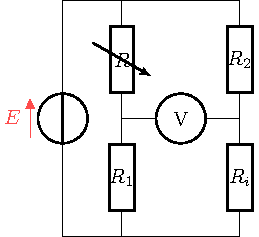
\includegraphics[width=\linewidth]{wheatstone-plain}
    \end{center}
\end{minipage}

\section{Ponts diviseurs de tension}
\begin{minipage}{0.50\linewidth}
    Donner les expressions de $U_1$, $U_2$, $U_3$ et $U_4$ en fonction de $E$ pour
les schémas suivants.\linebreak
\end{minipage}
\begin{minipage}{0.50\linewidth}
    \begin{tabularx}{\linewidth}{Y*{1}{Y}}
        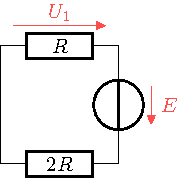
\includegraphics[scale=1]{pdt_a-plain} &
        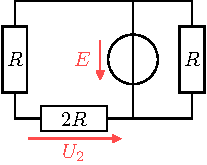
\includegraphics[scale=1]{pdt_b-plain}\\
        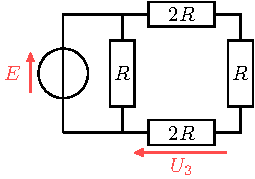
\includegraphics[scale=1]{pdt_c-plain} &
        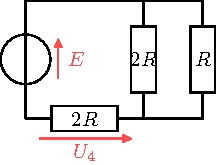
\includegraphics[scale=1]{pdt_d-plain}\\
    \end{tabularx}
\end{minipage}

\section{Pont diviseur de courant}
Exprimer l'intensité $I$ en fonction de $I_0$.
\begin{center}
    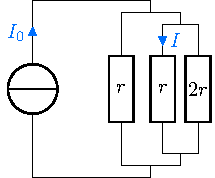
\includegraphics[scale=1]{divcour_last-plain}
\end{center}

\end{document}
